\section{Investigation}
\label{sec:investigation}
We now use POSE to investigate the CPU power consumption of codes taken from the Mantevo~\cite{heroux:2009aa} and Rodinia~\cite{che:2009aa} application suites.
The applications we study are all simplified versions of production codes intended for research purposes.
As such they exhibit relatively compact code bases and well understood behaviours while still providing represantative workloads.

CPU power consumption accounts for a significant portion of the energy used by high performance systems~\cite{rong:2010aa}, making it a prime candidate for optimisation.
Crucially for POSE, this variety of power consumption can be accurately measured on unmodified comodity hardware~\cite{hackenberg:2013aa}.

\subsection{CPU Power Consumption}
\label{ssec:cpupower}
Modern processors rely on Complimentary Metal Oxide Semiconductor (CMOS) technology.
\autoref{eq:totpwr} separates the power draw of CMOS chips into its component parts, of which dynamic power and leakage power are most significant.
\begin{equation}
\label{eq:totpwr}
P_{tot} = P_{dyn} + P_{leak} + P_{other}
\end{equation}
Dynamic power is consumed when logic gates change state as a processor performs work. 
Leakage power exists because at microscopic scales the insulating properties of silicon break down, allowing some current to escape even when gates remain inactive.
Other forms of power dissipation exist, however their effects are relatively minor \cite{kaxiras:2008aa}.
\begin{gather}
P_{dyn} \propto CV^{2}Af \label{eq:dynpwr} \\
P_{leak} = V \times I_{leak} \label{eq:staticpwr} \\
P_{tot} \propto CV^{2}Af + VI_{leak} \label{eq:totpwr2} 
\end{gather}
\autoref{eq:dynpwr} is a common approximation for dynamic power in which $C$ denotes load capacitance, $V$ the supply voltage, $A$ the activity factor and $f$ the clock frequency. 
\autoref{eq:staticpwr} is a simplified expression for leakage power that exploits the fact that leakage current $I_{leak}$ is invariant to processor workload~\cite{kim:2003aa}.
Substituting these into \autoref{eq:totpwr} yields the parametrised expression for total power consumption given in \autoref{eq:totpwr2} in which all terms except frequency, voltage and activity factor are constants.

Activity factor captures the fraction of logic elements which change state each clock cycle.
Frequency and supply voltage vary in tandem, taking values from a fixed set of $(frequency, voltage)$ pairs known as P-States.
Dynamic Voltage and Frequency Scaling (DVFS) selects the most appropriate P-State for the current workload.
Finally, capacitance and leakage current are constants dictated by processor design.

Processor architecture also plays a significant roll in determining total power consumption.
Each core in a multicore architecture operates independantly with its own activity factor and P-State.
As a result, \autoref{eq:totpwr2} should be summed across all cores to arrive at a value for the entire processor.

\subsection{Feasible Performance Envelope}
When applying POSE the first step is to construct an appropriate feasible performance envelope.
Processor manufacturers usually supply power consumption envelopes for their hardware, however these tend to be conservative estimates.
POSE works best when the maximum and minimum power bounds are as tight as possible, so instead we determine $P_{\alpha}$ and $P_{\beta}$ empirically. 

The properties we must account for when developing benchmarks for $P_{\alpha}$ and $P_{\beta}$ are P-State, activity factor and the number of cores active.
Of these, P-State is the easiest 

\clearpage


We define the range of values that activity factor can take while running a code as $[\alpha,~\beta]$ where $0 < \alpha < \beta < 1$. These values are a function of hardware design and for multi-core systems the number of cores active.


\todo{Flesh this out into some sort of abstract methodology.}
As previously discussed, activity factor and P-state are the only properties through which code (and hence performance engineers) can influence power consumption.
We use the \texttt{cpufrequtils} package to override DVFS and manually set the desired P-states, leaving only activity factor to consider.

\begin{figure}[ht]                                                               
\centering                                                                      
\lstset{basicstyle=\ttfamily\footnotesize\bfseries, frame=tb} %small bold text, lines top and bottom 
\lstinputlisting[]{lst/alpha_benchmark.c}              
\caption{Baseline Power Micro-Benchmark}                            
\label{fig:microbench}                                                           
\end{figure}  

Our benchmark for activity factor $\alpha$ is given in \autoref{fig:microbench}.
It repeatedly executes a single \texttt{jmp} instruction, performing no computation or memory accesses in the process.
We assert that non-trivial computational workloads exhibit strictly higher activity factors than this minimal micro-benchmark.
The only exceptions are applications which spend so long blocked waiting for resources they allow the processor to enter idle states.
If necessary this behaviour can be captured by adding corresponding delays to the benchmark.

We evaluated three codes
Prime95 and Linpack are two codes frequently used to stress-test CPU power consumption.

We also evaluated Prime95 and Linpack as potential $P_{\beta}$ benchmarks


before settling on FIRESTARTER.

FIRESTARTER~\cite{hackenberg:2013ab}, a tool designed to trigger near-peak power consumption in a range of x86\_64 processors.

compute nodes.

FIRESTARTER, `a simple yet versatile tool that generates near-peak power consumption of compute nodes'.
We evaluated several stress test tools in order to benchmark $P_{\beta}$ before we settled on
FIRESTARTER, which is 
We use FIRESTARTER, a benchmark

\begin{enumerate}
  \item \todo{(Abstract) Methodology - say we just measure for $\{freq\} \times \{cores\}$}
  \item \todo{FIRESTARTER $\beta$ paragraph}
  \item \todo{Experimental Setup}
  \begin{enumerate}
    \item \todo{Get hardware deets from camelot}
  \end{enumerate}
  \item \todo{Write up results}
  \item \todo{Bosh out freq comparison waffle}
\end{enumerate}


\todo{WORKING POINT}

Linpack is characterised by its extremely high code intensity. 
\todo{false baselines etc}
This highlights the fact that effective use of POSE depends largely on the choice of roofline and 


\begin{table}
\centering
\caption{Early Investigation}
\input{tab/tex/code_metrics.tex}
\end{table} 



  \begin{table}
    \setlength{\tabcolsep}{.5em}
    \caption{Code POSE Values}
    \begin{subtable}{\textwidth}
    \centering
    \caption{Time (s)}
    \input{tab/tex/code_pose_time.tex}
    \end{subtable} 
    \begin{subtable}{\textwidth}
    \centering
    \caption{Energy (J)}
    \input{tab/tex/code_pose_energy.tex}
    \end{subtable}
    \label{tab:pose_params}
  \end{table} 



\subsection{Experimental Methodology}
CPU energy consumption was measured using Intel's Running Average Power Limit (RAPL) technology~\cite{david:2010aa}.
We created a simple tool babsed on the Unix \texttt{time} which output energy consumption figures as well as conventional runtime figures.
The techniques described in \cite{hahnel:2012aa} were used to ensure measurement accuracy. 

\todo{Detail app arguments etc.}


\todo{consider each in turn as a potential source of optimisations.}
%TODO make sure this is explicitly Linpack table in text
\begin{table}
\centering
\caption{Feasible Performance Envelope Parameters (W)}
\input{tab/tex/fpe_params.tex}
\end{table} 

\begin{figure}[t]%
  \providecommand{\plotwidth}{.95\linewidth}
  \begin{subfigure}[t]{.5\linewidth}%
    \begin{tikzpicture}
  \begin{axis}[
    axis on top,
    axis x line=bottom,
    axis y line=left,
    xlabel={Runtime (\emph{s})},
    ylabel={Energy (\emph{J})},    
    xmin=24, xmax=31,
    ymin=650, ymax=1650,
    width=0.80\linewidth,
    legend columns=3,
    legend to name=minimd:legend,
    legend style={/tikz/every even column/.append style={column sep=0.2cm}} % space out columns a bit
    ]

    %% Model Parameters %%
    \pgfmathsetmacro{\baselinepower}{26.876067}
    \pgfmathsetmacro{\rooflinepower}{49.60612}
    \pgfmathsetmacro{\codepower}{27.95947000000066} 
    \pgfmathsetmacro{\codetime}{30.293834}
    \pgfmathsetmacro{\codeenergy}{846.999542908}
    \pgfmathsetmacro{\energyexp}{1.0}
    \pgfmathsetmacro{\timeexp}{2.0}

    % Sadly, pgfplots sucks too much to calculate cube roots
    % These values are calculated with a ruby script in tools
    \pgfmathsetmacro{\blnodex}{29.897382525363728}
    \pgfmathsetmacro{\brnodex}{30.69554258273286}
    \pgfmathsetmacro{\trnodex}{25.0237350439618}
    \pgfmathsetmacro{\tlnodex}{24.373056016397907}

    %% Intermezzo Values %%
    \pgfmathsetmacro{\brnodey}{\brnodex * \baselinepower}
    \pgfmathsetmacro{\blnodey}{\blnodex * \baselinepower}
    \pgfmathsetmacro{\tlnodey}{\tlnodex * \rooflinepower}
    \pgfmathsetmacro{\trnodey}{\trnodex * \rooflinepower}
    \pgfmathsetmacro{\codeenergy}{\codepower * \codetime}
    \pgfmathsetmacro{\baselineenergy}{\baselinepower * \codetime}

    % arguments: code power, code time, x - todo, apparently not supposed to do pgfmathparse
    \pgfmathdeclarefunction{metricbound}{3}{%
      \pgfmathparse{((#1 * #2^3) / #3^2)}%
    }
    \pgfmathdeclarefunction{definitionbound}{3}{%
      \pgfmathparse{((#1 / #2^3) * #3^4)}%
    }

   % BETA ROOFLINE BOUND 
    \addplot[color=printred, very thick, domain=\pgfkeysvalueof{/pgfplots/xmin}:\pgfkeysvalueof{/pgfplots/xmax}] {\rooflinepower * x};
    \addlegendentry{$P_{max}$ Energy Bound}

    % ALPHA BASELINE BOUND 
    \addplot[color=printgreen, very thick, domain=\pgfkeysvalueof{/pgfplots/xmin}:\pgfkeysvalueof{/pgfplots/xmax}] {\baselinepower * x};
    \addlegendentry{$P_{min}$ Energy Bound} 

    \addplot[color=printorange, domain=\trnodex:\brnodex] { metricbound(\codepower, \codetime, x)};
    \addlegendentry{Optimisation Bound}

    \addplot[color=printblue, domain=\blnodex:\codetime] { definitionbound(\codepower, \codetime, x)};
    \addlegendentry{Contribution Bound}

    \addplot[color=printorange, densely dashed, domain=\tlnodex:\blnodex] {metricbound(\baselinepower, \blnodex, x)};
    \addlegendentry{Optimisation Limit}

    % Constant Time (Vertical) dotted line
    \draw[densely dotted] ({axis cs:\codetime,\baselineenergy}) -- ({axis cs:\codetime,\codeenergy});

    \node[circle,fill,inner sep=1pt] at (axis cs:\codetime,\codeenergy) {};
    \node[above right] at (axis cs:\codetime,\codeenergy) {$\theta$};
    
    \node [above] at ({axis cs:\tlnodex, \tlnodey}) {A};
    \node [above] at ({axis cs:\trnodex, \trnodey}) {B};
    \node [below] at ({axis cs:\blnodex, \blnodey}) {C};
    \node [below] at ({axis cs:\codetime,\baselineenergy}) {D};
    \node [below] at ({axis cs:\brnodex, \brnodey}) {E};
 \end{axis}
\end{tikzpicture}
%
    \caption{MiniMD}%
  \end{subfigure}%
  \begin{subfigure}[t]{.5\linewidth}%
    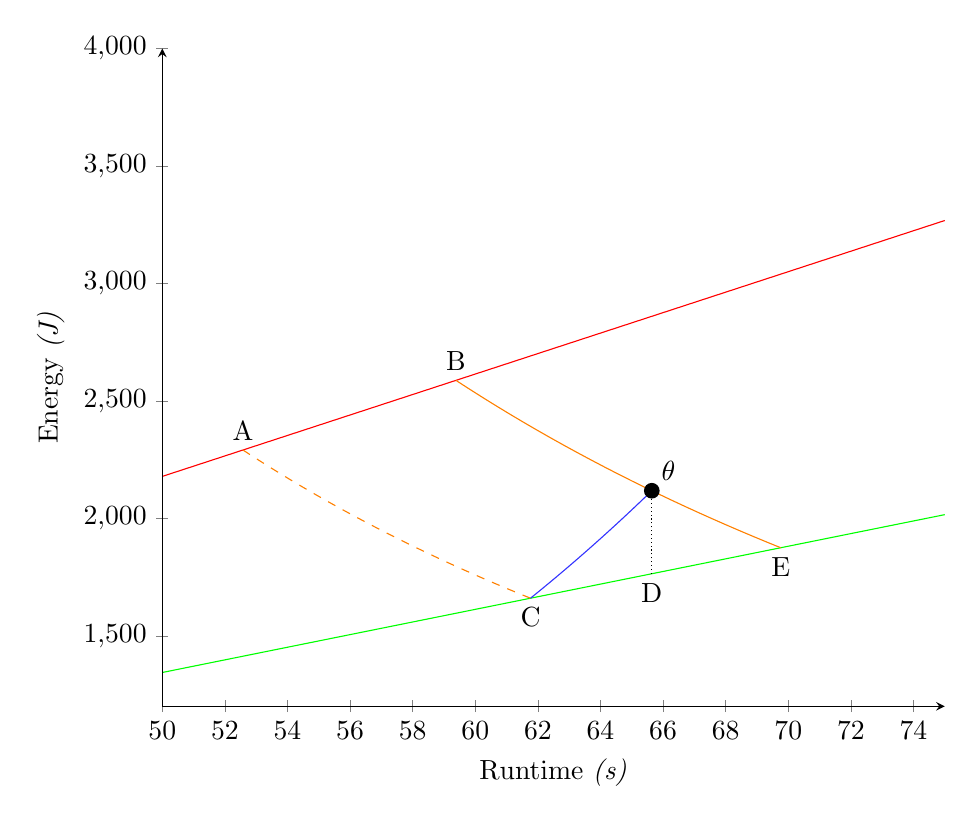
\begin{tikzpicture}
  \providecommand{\plotwidth}{\linewidth}
  \begin{axis}[
    axis on top,
    axis x line=bottom,
    axis y line=left,
  	xlabel={Runtime \emph{(s)}},
    ylabel={Energy \emph{(J)}},    
    xmin=50, xmax=75,
    ymin=1200, ymax=4000,
    width=\plotwidth,
    legend to name=lavamd:legend
    ]

    %% Model Parameters %%
    \pgfmathsetmacro{\baselinepower}{26.876067}
    \pgfmathsetmacro{\rooflinepower}{43.570651}
    \pgfmathsetmacro{\codepower}{32.259372}
    \pgfmathsetmacro{\codetime}{65.640072}
    % Sadly, pgfplots sucks too much to calculate cube roots
    % These values are calculated with a ruby script in tools
    \pgfmathsetmacro{\brnodex}{69.75881800188515}
    \pgfmathsetmacro{\blnodex}{61.764507707810466}
    \pgfmathsetmacro{\trnodex}{59.38220710689976}
    \pgfmathsetmacro{\tlnodex}{52.57704894686994}
    
    %% Intermezzo Values %%
    \pgfmathsetmacro{\brnodey}{\brnodex * \baselinepower}
    \pgfmathsetmacro{\blnodey}{\blnodex * \baselinepower}
    \pgfmathsetmacro{\tlnodey}{\tlnodex * \rooflinepower}
    \pgfmathsetmacro{\trnodey}{\trnodex * \rooflinepower}
    \pgfmathsetmacro{\codeenergy}{\codepower * \codetime}
    \pgfmathsetmacro{\baselineenergy}{\baselinepower * \codetime}

    % arguments: code power, code time, x - todo, apparently not supposed to do pgfmathparse
    \pgfmathdeclarefunction{metricbound}{3}{%
      \pgfmathparse{((#1 * #2^3) / #3^2)}%
    }
    \pgfmathdeclarefunction{definitionbound}{3}{%
      \pgfmathparse{((#1 / #2^3) * #3^4)}%
    }

    % BETA ROOFLINE BOUND 
    \addplot[color=red, domain=\pgfkeysvalueof{/pgfplots/xmin}:\pgfkeysvalueof{/pgfplots/xmax}] {\rooflinepower * x};
    \addlegendentry{$P_{max}$ Energy Bound}

    % ALPHA BASELINE BOUND 
    \addplot[color=green, domain=\pgfkeysvalueof{/pgfplots/xmin}:\pgfkeysvalueof{/pgfplots/xmax}] {\baselinepower * x};
    \addlegendentry{$P_{min}$ Energy Bound} 

    \addplot[color=orange, domain=\trnodex:\brnodex] { metricbound(\codepower, \codetime, x)};
    \addlegendentry{Optimisation Bound}

    \addplot[color=blue!80, domain=\blnodex:\codetime] { definitionbound(\codepower, \codetime, x)};
    \addlegendentry{Contribution Bound}

    \addplot[color=orange, dashed, domain=\tlnodex:\blnodex] {metricbound(\baselinepower, \blnodex, x)};
    \addlegendentry{Optimisation Limit}

    % Constant Time (Vertical) dotted line
    \draw[densely dotted] ({axis cs:\codetime,\baselineenergy}) -- ({axis cs:\codetime,\codeenergy});

    \node[circle,fill,inner sep=2pt] at (axis cs:\codetime,\codeenergy) {};
    \node[above right] at (axis cs:\codetime,\codeenergy) {$\theta$};
    
    \node [above] at ({axis cs:\tlnodex, \tlnodey}) {A};
    \node [above] at ({axis cs:\trnodex, \trnodey}) {B};
    \node [below] at ({axis cs:\blnodex, \blnodey}) {C};
    \node [below] at ({axis cs:\codetime,\baselineenergy}) {D};
    \node [below] at ({axis cs:\brnodex, \brnodey}) {E};
 \end{axis}
\end{tikzpicture}
%
    \caption{LavaMD}%
  \end{subfigure}%
  \begin{center}%
    \ref{minimd:legend}%
  \end{center}%
  \caption{$E^1t^2$ POSE for Activity Factor Optimisation}%
  \label{fig:minimd}%
\end{figure}

\begin{figure}[t]%
\begin{subfigure}[t]{.5\linewidth}%
\centering%
\@ifundefined{pstateminimdtable}{%
  \pgfplotstableread[col sep=comma]{plot/minimd-pstates/data/pstate_power_4_cores.csv}\pstateminimdtable
}{}

\begin{tikzpicture}
  \begin{axis}[
    width=0.75\linewidth,
    axis on top,
    axis x line=bottom,
    axis y line=left,
    xlabel={Runtime (\emph{s})},
    ylabel={Energy (\emph{J})},    
    xmin=20, xmax=65,
    ymin=200, ymax=1200,
    legend columns=2,
    legend to name=minimd-pstate:legend,
    legend style={/tikz/every even column/.append style={column sep=0.2cm}} % space out columns a bit
    ]

    % arguments: code power, code time, x, n 
    \pgfmathdeclarefunction{metricbound}{4}{%
      \pgfmathparse{((#1 * #2^(#4 + 1)) / #3^#4)}%
    }
    \pgfmathdeclarefunction{definitionbound}{4}{%
      \pgfmathparse{((#1 / #2^(#4 + 1)) * #3^(#4 + 2))}%
    }

    %%
    \pgfmathsetmacro{\codetime}{31.160996}
    \pgfmathsetmacro{\codepower}{26.555410070974624}
    \pgfmathsetmacro{\blnodex}{24.876044579784466}
    \addplot[black, densely dotted, domain=\blnodex:\codetime, forget plot] {definitionbound(\codepower, \codetime, x, 2)};

    %%
    \pgfmathsetmacro{\codetime}{32.221644}
    \pgfmathsetmacro{\codepower}{25.19066851461707}
    \pgfmathsetmacro{\blnodex}{26.17914532437151}
    \addplot[black, densely dotted, domain=\blnodex:\codetime, forget plot] {definitionbound(\codepower, \codetime, x, 2)};

    %%
    \pgfmathsetmacro{\codetime}{33.189564}
    \pgfmathsetmacro{\codepower}{24.052689996168674}
    \pgfmathsetmacro{\blnodex}{27.384280155637242}
    \addplot[black, densely dotted, domain=\blnodex:\codetime, forget plot] {definitionbound(\codepower, \codetime, x, 2)};

    %%
    \pgfmathsetmacro{\codetime}{35.548669}
    \pgfmathsetmacro{\codepower}{21.708309894809283}
    \pgfmathsetmacro{\blnodex}{30.35072062021389}
    \addplot[black, densely dotted, domain=\blnodex:\codetime, forget plot] {definitionbound(\codepower, \codetime, x, 2)};

    %%
    \pgfmathsetmacro{\codetime}{36.852917}
    \pgfmathsetmacro{\codepower}{20.791885293639034}
    \pgfmathsetmacro{\blnodex}{31.919904165043228}
    \addplot[black, densely dotted, domain=\blnodex:\codetime, forget plot] {definitionbound(\codepower, \codetime, x, 2)};

    %%
    \pgfmathsetmacro{\codetime}{38.225746}
    \pgfmathsetmacro{\codepower}{19.926273930664426}
    \pgfmathsetmacro{\blnodex}{33.58161699951163}
    \addplot[black, densely dotted, domain=\blnodex:\codetime, forget plot] {definitionbound(\codepower, \codetime, x, 2)};

    %%
    \pgfmathsetmacro{\codetime}{39.720356}
    \pgfmathsetmacro{\codepower}{19.032817706870503}
    \pgfmathsetmacro{\blnodex}{35.432334683311204}
    \addplot[black, densely dotted, domain=\blnodex:\codetime, forget plot] {definitionbound(\codepower, \codetime, x, 2)};

    %%
    \pgfmathsetmacro{\codetime}{41.430395}
    \pgfmathsetmacro{\codepower}{18.26008617586195}
    \pgfmathsetmacro{\blnodex}{37.47190734697387}
    \addplot[black, densely dotted, domain=\blnodex:\codetime, forget plot] {definitionbound(\codepower, \codetime, x, 2)};

    %%
    \pgfmathsetmacro{\codetime}{45.85507}
    \pgfmathsetmacro{\codepower}{16.61222678321067}
    \pgfmathsetmacro{\blnodex}{42.802165661611}
    \addplot[black, densely dotted, domain=\blnodex:\codetime, forget plot] {definitionbound(\codepower, \codetime, x, 2)};

    %%
    \pgfmathsetmacro{\codetime}{49.7305}
    \pgfmathsetmacro{\codepower}{15.67846259337831}
    \pgfmathsetmacro{\blnodex}{47.323406701270244}
    \addplot[black, densely dotted, domain=\blnodex:\codetime, forget plot] {definitionbound(\codepower, \codetime, x, 2)};

    %%
    \pgfmathsetmacro{\codetime}{52.358683}
    \pgfmathsetmacro{\codepower}{15.137478343372388}
    \pgfmathsetmacro{\blnodex}{50.41098720057872}
    \addplot[black, densely dotted, domain=\blnodex:\codetime, forget plot] {definitionbound(\codepower, \codetime, x, 2)};

    %%
    \pgfmathsetmacro{\codetime}{55.340763}
    \pgfmathsetmacro{\codepower}{14.650088958838532}
    \pgfmathsetmacro{\blnodex}{53.866578212248804}
    \addplot[black, densely dotted, domain=\blnodex:\codetime, forget plot] {definitionbound(\codepower, \codetime, x, 2)};

    %%
    \pgfmathsetmacro{\codetime}{58.637567}
    \pgfmathsetmacro{\codepower}{14.09304050763225}
    \pgfmathsetmacro{\blnodex}{57.81786383949271}
    \addplot[black, densely dotted, domain=\blnodex:\codetime, forget plot] {definitionbound(\codepower, \codetime, x, 2)};


    %% Model Parameters %%
    \pgfplotstablegetelem{0}{Runtime}\of{\pstateminimdtable}
    \pgfmathsetmacro{\codetime}{\pgfplotsretval} 
    \pgfplotstablegetelem{0}{Energy}\of{\pstateminimdtable}
    \pgfmathsetmacro{\codeenergy}{\pgfplotsretval} 
    \pgfmathsetmacro{\baselinepower}{13.510238}

    %% Intermezzo Values %%
    \pgfmathsetmacro{\codepower}{\codeenergy / \codetime}



    % ALPHA BASELINE BOUND 
    \addplot[color=printgreen, very thick, name path=basebound, domain=\pgfkeysvalueof{/pgfplots/xmin}:\pgfkeysvalueof{/pgfplots/xmax}] {\baselinepower * x};
    \addlegendentry{$P_{min}$ Energy Bound} 


    %% 3.2 GHz start point
    \pgfmathsetmacro{\blnodex}{23.77199310523716}
    \pgfmathsetmacro{\brnodex}{38.6049404590049}
    \addplot[name path=edpdef, darkgray, thick, domain=\blnodex:\codetime, forget plot] {definitionbound(\codepower, \codetime, x, 2)};
    \addplot[name path=edpopt, darkgray, thick, domain=\codetime:\brnodex] {metricbound(\codepower, \codetime, x, 2)};
    \addlegendentry{3.2 GHz POSE}

    % 2.2 GHz non-overlapping pose
    \pgfmathsetmacro{\codetime}{43.161913}
    \pgfmathsetmacro{\codepower}{17.552650110758528}
    \pgfmathsetmacro{\blnodex}{39.55555231782452}
    \pgfmathsetmacro{\brnodex}{47.097072968441026}
    \addplot[name path=edpdef, gray, thick, domain=\blnodex:\codetime, forget plot] {definitionbound(\codepower, \codetime, x, 2)};
    \addplot[name path=edpopt, gray, thick, domain=\codetime:\brnodex] {metricbound(\codepower, \codetime, x, 2)};
    \addlegendentry{First Non-Overlapping POSE}
    
    %% PState progression
    \tikzset{ every pin edge/.append style={thick} }
    \addplot[mark=x, black, only marks] table[x=Runtime,y=Energy, trim cells=true] {\pstateminimdtable}
      node[pos=0.0, pin=above:3.2 GHz]{}
      node[pos=1.0, pin=above:1.6 GHz]{}
      node[pos=0.64285714285, pin=above:2.2 GHz]{} % pos is elem index / rows - 1 (zero indexed)
      % How to specify pin length (.15cm) and angle (120)
      %node[pos=0.5745, pin={[pin distance=0.15cm] 120:2.2 GHz}]{}
    ;
    \addlegendentry{P-state Measurement}
 \end{axis}
\end{tikzpicture}
%
\caption{MiniMD}%
\end{subfigure}%
\begin{subfigure}[t]{.5\linewidth}%
\@ifundefined{pstatelavamdtable}{%
  \pgfplotstableread[col sep=comma]{plot/lavamd-pstates/data/pstate_power_4_cores.csv}\pstatelavamdtable
}{}

\begin{tikzpicture}
  \begin{axis}[
    width=0.95\linewidth,
    axis on top,
    axis x line=bottom,
    axis y line=left,
  	xlabel={Runtime \emph{(s)}},
    ylabel={Energy \emph{(J)}},    
    xmin=0, xmax=140,
    ymin=0, ymax=3800,
    legend columns=2,
    legend to name=lavamd-pstate:legend,
    legend style={/tikz/every even column/.append style={column sep=0.2cm}} % space out columns a bit
    ]

    %% Model Parameters %%
    \pgfplotstablegetelem{0}{Runtime}\of{\pstatelavamdtable}
    \pgfmathsetmacro{\codetime}{\pgfplotsretval} 
    \pgfplotstablegetelem{0}{Energy}\of{\pstatelavamdtable}
    \pgfmathsetmacro{\codeenergy}{\pgfplotsretval} 
    \pgfmathsetmacro{\baselinepower}{13.510238}

    %% Intermezzo Values %%
    \pgfmathsetmacro{\codepower}{\codeenergy / \codetime}

    % arguments: code power, code time, x, n 
    \pgfmathdeclarefunction{metricbound}{4}{%
      \pgfmathparse{((#1 * #2^(#4 + 1)) / #3^#4)}%
    }
    \pgfmathdeclarefunction{definitionbound}{4}{%
      \pgfmathparse{((#1 / #2^(#4 + 1)) * #3^(#4 + 2))}%
    }

    % ALPHA BASELINE BOUND 
    \addplot[color=green, name path=basebound, domain=\pgfkeysvalueof{/pgfplots/xmin}:\pgfkeysvalueof{/pgfplots/xmax}] {\baselinepower * x};
    \addlegendentry{$P_{min}$ Energy Bound} 


    %% 3.2 GHz start point
    \pgfmathsetmacro{\brnodex}{87.73374843784023}
    \pgfmathsetmacro{\blnodex}{49.11016716922632}
    \addplot[name path=edpdef, draw=none, domain=\blnodex:\codetime+1, forget plot] {definitionbound(\codepower, \codetime, x, 2)};
    \addplot[name path=edpopt, draw=none, domain=\codetime-1:\brnodex, forget plot] {metricbound(\codepower, \codetime, x, 2)};

    \path[name path=edpspace,
      intersection segments={
        of=edpdef and edpopt,
        sequence=A0 -- B1,
      }
      ]; 
    \addplot[blue!20] fill between[of=edpspace and basebound]; 
    \addlegendentry{3.2 GHz POSE}

    %% PState progression
    \addplot[mark=x, black] table[x=Runtime,y=Energy, trim cells=true] {\pstatelavamdtable}
      node[pos=0.0, pin=left:3.2 GHz]{}
      node[pos=1.0, pin=95:1.6 GHz]{}
      node[pos=0.636, pin={[pin distance=0.15cm] above:2.1 GHz}]{}
    ;
    \addlegendentry{P-State Progression}


    %%
    \pgfmathsetmacro{\codetime}{67.788671}
    \pgfmathsetmacro{\codepower}{30.534496154969613}
    \pgfmathsetmacro{\blnodex}{51.65525781584337}
    \addplot[name path=edpdef, gray, densely dashed, domain=\blnodex:\codetime, forget plot] {definitionbound(\codepower, \codetime, x, 2)};

    %%
    \pgfmathsetmacro{\codetime}{69.909725}
    \pgfmathsetmacro{\codepower}{28.972621505806238}
    \pgfmathsetmacro{\blnodex}{54.21207070239038}
    \addplot[name path=edpdef, gray, densely dashed, domain=\blnodex:\codetime, forget plot] {definitionbound(\codepower, \codetime, x, 2)};

    %%
    \pgfmathsetmacro{\codetime}{72.820343}
    \pgfmathsetmacro{\codepower}{27.23156518227331}
    \pgfmathsetmacro{\blnodex}{57.647815146592066}
    \addplot[name path=edpdef, gray, densely dashed, domain=\blnodex:\codetime, forget plot] {definitionbound(\codepower, \codetime, x, 2)};

    %%
    \pgfmathsetmacro{\codetime}{78.83738}
    \pgfmathsetmacro{\codepower}{24.363863791516156}
    \pgfmathsetmacro{\blnodex}{64.76958711476986}
    \addplot[name path=edpdef, gray, densely dashed, domain=\blnodex:\codetime, forget plot] {definitionbound(\codepower, \codetime, x, 2)};

    %%
    \pgfmathsetmacro{\codetime}{80.443575}
    \pgfmathsetmacro{\codepower}{23.569310575766927}
    \pgfmathsetmacro{\blnodex}{66.82363092159444}
    \addplot[name path=edpdef, gray, densely dashed, domain=\blnodex:\codetime, forget plot] {definitionbound(\codepower, \codetime, x, 2)};

    %%
    \pgfmathsetmacro{\codetime}{83.583275}
    \pgfmathsetmacro{\codepower}{22.42571518045925}
    \pgfmathsetmacro{\blnodex}{70.59245458487962}
    \addplot[name path=edpdef, gray, densely dashed, domain=\blnodex:\codetime, forget plot] {definitionbound(\codepower, \codetime, x, 2)};

    %%
    \pgfmathsetmacro{\codetime}{87.25231}
    \pgfmathsetmacro{\codepower}{21.415643975500476}
    \pgfmathsetmacro{\blnodex}{74.83203474018039}
    \addplot[name path=edpdef, gray, densely dashed, domain=\blnodex:\codetime, forget plot] {definitionbound(\codepower, \codetime, x, 2)};

    %%
    \pgfmathsetmacro{\codetime}{90.581583}
    \pgfmathsetmacro{\codepower}{20.54295973167084}
    \pgfmathsetmacro{\blnodex}{78.77224707386881}
    \addplot[name path=edpdef, gray, densely dashed, domain=\blnodex:\codetime, forget plot] {definitionbound(\codepower, \codetime, x, 2)};

    %%
    \pgfmathsetmacro{\codetime}{95.357508}
    \pgfmathsetmacro{\codepower}{19.637888418812288}
    \pgfmathsetmacro{\blnodex}{84.1803958382032}
    \addplot[name path=edpdef, gray, densely dashed, domain=\blnodex:\codetime, forget plot] {definitionbound(\codepower, \codetime, x, 2)};

    %%
    \pgfmathsetmacro{\codetime}{99.502899}
    \pgfmathsetmacro{\codepower}{18.820670933416725}
    \pgfmathsetmacro{\blnodex}{89.0932975465577}
    \addplot[name path=edpdef, red, densely dashed, domain=\blnodex:\codetime] {definitionbound(\codepower, \codetime, x, 2)};
    \addlegendentry{Optimisation Cutoff}
    %%
    \pgfmathsetmacro{\codetime}{109.970804}
    \pgfmathsetmacro{\codepower}{17.334285425429826}
    \pgfmathsetmacro{\blnodex}{101.20370662532102}
    \addplot[name path=edpdef, gray, densely dashed, domain=\blnodex:\codetime, forget plot] {definitionbound(\codepower, \codetime, x, 2)};

    %%
    \pgfmathsetmacro{\codetime}{115.469869}
    \pgfmathsetmacro{\codepower}{16.703561489274747}
    \pgfmathsetmacro{\blnodex}{107.58539357794623}
    \addplot[name path=edpdef, gray, densely dashed, domain=\blnodex:\codetime, forget plot] {definitionbound(\codepower, \codetime, x, 2)};

    %%
    \pgfmathsetmacro{\codetime}{123.182269}
    \pgfmathsetmacro{\codepower}{16.060352379123653}
    \pgfmathsetmacro{\blnodex}{116.28334319474206}
    \addplot[name path=edpdef, gray, densely dashed, domain=\blnodex:\codetime, forget plot] {definitionbound(\codepower, \codetime, x, 2)};

    %%
    \pgfmathsetmacro{\codetime}{130.924339}
    \pgfmathsetmacro{\codepower}{15.486518591474423}
    \pgfmathsetmacro{\blnodex}{125.09985043035239}
    \addplot[name path=edpdef, gray, densely dashed, domain=\blnodex:\codetime, forget plot] {definitionbound(\codepower, \codetime, x, 2)};
  \end{axis}
\end{tikzpicture}
%
\caption{LavaMD}%
\end{subfigure}%
\begin{center}%
\ref{minimd-pstate:legend}%
\end{center}%
\caption{$E^1t^2$ POSE for P-State Optimisation}%
\label{fig:pstates}%
\end{figure}%

Changes in processor P-State do not effect code performance linearly due to system bottlenecks. Critical path? \todo{is there a smart term for this? Bound and bottleneck analysis.} A modern super-scalar CPU contains many specialized functional units. A code which is bottlenecked by Memory accesses may when slowed dow.

A code with low operational intensity 


\subsection{Results}


\autoref{tab:pose_params} \todo{reword given central table} shows that for MiniMD, the longest runtime within the Power Optimized Software Envelope is 30.70s.
This means that any optimization which trades increased runtime for improved power efficiency can slow MiniMD down by at most 0.41s before $E^1t^2$ becomes strictly worse.
The upper limit of energy to be saved from power optimisation alone for MiniMD running on our target platform is is 32.82J.
The lowest value of $E^1t^2$ within the envelope is 718232.78, an improvement of 7.60\% over the baseline code. 
Runtime optimization will be required to deliver any improvements above this level.
We also know that a speedup of, 1.16x, or 4.16s, is guaranteed to beat $\theta$ in terms of $E^1t^2$.
Finally, a speedup of 1.19x, or 4.84s, is guaranteed to beat any power optimised version of $\theta$ in terms of $E^1t^2$

\autoref{tab:pose_params} \todo{reword given central} shows that for LavaMD, the longest runtime within the Power Optimized Software Envelope as 69.76s.
This means that any optimization which trades increased runtime for improved power efficiency can slow LavaMD down by at most 4.12s before $E^1t^2$ becomes strictly worse.
The upper limit of energy to be saved from power optimization alone is 353.36J.
The lowest value of $E^1t^2$ within the envelope is 6332608.91, an improvement of 30.59\% over the baseline code.
Runtime optimization will be required to deliver any improvements above this level.
We also know that a speedup of 1.11x, or 6.26s, is guaranteed to beat $\theta$ in terms of $E^1t^2$.
Finally, a runtime optimisation of 1.25x, or 13.06s, is guaranteed to beat any power optimised version of $\theta$ in terms of $E^1t^2$ 

\subsection{Discussion}

\todo{both in absolute terms and as a percentage of the baseline}

The figures produced by POSE are all upper bounds, and the benefits of power optimisation will be more modest in practice. Even so, these figures are useful as they allow performance engineers to make informed decisions about where best to focus their efforts. If they consider a $1.03 \times$ speed up to be more achievable than up to the maximum $1.17\times$ reduction in activity factor then they can proceed to apply conventional optimisations safe in the knowledge that overall performance will improve despite any increases in activity factor.

If a performance engineer decides the benefits of power optimisation are worth pursuing after applying POSE, the question still remains as to how he should go about searching for those optimisations.
